\subsection{Grobkonzept 3} \label{subsec:grobkonzept3}
\begin{table}[H]
\footnotesize
\begin{tabular}{>{\HY\RaggedRight}p{3cm} >{\HY\RaggedRight}p{2.2cm} >{\HY\RaggedRight}p{4cm} >{\HY\RaggedRight}p{3.3cm} >{\HY\RaggedRight}p{1.2cm}}
\hline
	\textbf{Bestandteil}		&\textbf{Typ}			&\textbf{Funktion}									&\textbf{Specs}			&\textbf{Anz.}\\
	\hline
\rowcolor{dgelb}
\multicolumn{5}{l}{\textbf{Stromerzeugung}}\\
	Turbine 					&Pelton 					&Umwandlung in Rotationsenergie						&							&5	\\
	Generator				&						&Umwandlung in elektrische Energie					&							&5	\\
\rowcolor{dblau}
\multicolumn{5}{l}{\textbf{Elektrotechnik}}\\
 	Wechselrichter			&						&Einspeisung ins Stromnetz							&							&1	\\
 	Ventilsteuerung			&						&Öffnet/schliesst Ventile je nach Füllstand			&							&1	\\
\rowcolor{dpink}
\multicolumn{5}{l}{\textbf{Bedienung}}\\
 	Anzeige 					&LCD-Display				&zeigt Tankfüllstände und die Generatordaten an 		&							&1	\\
 	Alarmleuchte				&						&Warnt bei zu hochem Füllstand in einem der Tanks 	&							&1	\\
\rowcolor{dgruen}
\multicolumn{5}{l}{\textbf{Abwassertechnik}}\\
	Tanks 					& 						&Zwischenspeicher für Abwasser 						&4m\textsuperscript{3}, trichterförmig		&5 	\\
	Ablassventil				&						&Entlässt das Abwasser aus dem Tank 					&							&5	\\
	Entlüftung				&						&ermöglicht Luftaustausch, entlässt Gase				&							&5	\\
	Notüberlauf				&						&Verhindert, dass Tank zu voll wird					&							&5	\\
	Füllstandsensor			&Ultraschall				&Misst den Füllstand des Tanks						&Messbereich <20cm bis >3m	&5	\\
	Druckleitungen			&						&Machen hohe Wassersäulen möglich?					&Druckfestigkeit >40 bar	&5	\\
	Bypass für Turbinen 		&Manuell					&ermöglicht Wartung der Turbine 						&							&5	\\
	Bypass für Tanks 		&Manuell					&ermöglicht Wartung und Reingung der Tanks 			&	 						&5	\\ 
\hline
\end{tabular}
\end{table}
\newpage
\begin{wrapfigure}{r}{0.5\textwidth}
  \begin{center}
    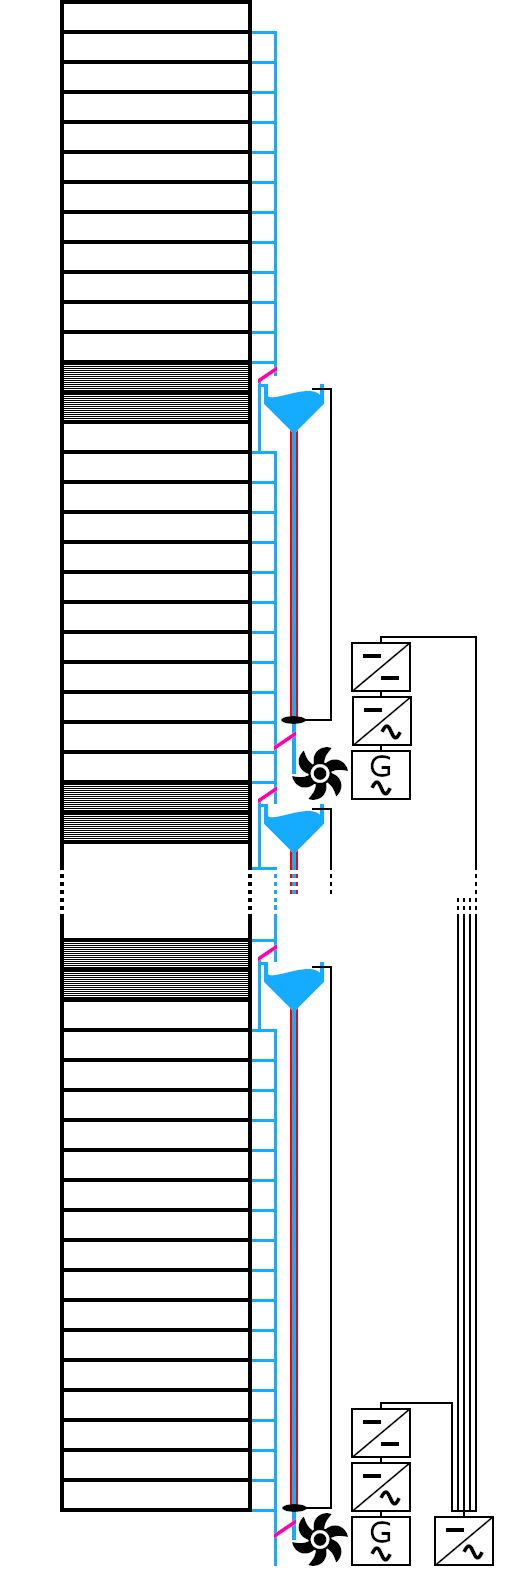
\includegraphics[width=0.48\textwidth]{grobkonzept3}
  \end{center}
  \caption{Grobkonzept 3}
\end{wrapfigure}
Dieses Grobkonzept ist fast identisch zu Grobkonzept 2. Es gibt wieder mehrere Tanks in einem Abstand von 14 Stockwerken, in denen das Abwasser zwischengespeichert wird. Allerdings gibt es nicht nur eine, sondern gleich viele Turbinen wie Tanks. Das Abwasser fliesst von einem Tank 14 Stockwerke nach unten, durch eine Turbine und dann in den nächsten Tank. Bei Grobkonzept 2 kann es unter Umständen relativ lange dauern, bis die Rohre komplett mit Wasser gefüllt sind. Bis das der Fall ist, kommt es zu Luftwiderstand in der Leitung, der das Abwasser abbremst. Bei jedem Tank eine Turbine einzubauen hat den Vorteil, dass die Rohre kürzer sind und so nach öffnen des Ventils schneller komplett mit Wasser gefüllt werden. So wird die Zeit verkürzt, in der Luftwiderstand auftritt. Ausserdem ist der Druck in den Leitungen geringer, man kann also günstigere Rohre und Ventile verwenden. Da im Vergleich zu Grobkonzept 2 keinen Rückstau geben kann, ist es nicht nötig, Einwegventile in die Druckleitung einzubauen. 

\textbf{Vorteile:} 									\newline
+	Luftwiderstand tritt kürzer auf 				\newline
+	Weniger Druck in den Leitungen					\newline

\textbf{Nachteile:}									\newline
-	Braucht viel Platz								\newline
-	Grössere bauliche Massnahmen nötig				\newline
-	Verstopfungsgefahr								\newline
-	Mehrere Turbinen nötig
\WFclear			
\newpage